% @file load_data.tex
% @project IAL Náhradní projekt - 05. Rovinnost grafu
% @author Vladimir Meciar (xmecia00), Ondrej Podrouzek (xpodro03)
% @brief This file is module for documentation.tex with documantation for scanner
% @changes 7.12.2022
\section{Nacitanie dat}

\subsection{Vstupne data}
Struktura ktoru potrebujeme nacitat (graf), je definovana ako mnozina vrcholov a hran vrcholov. Pre nase potreby
sme pouzili ulozenie v texte s predpisanym formatom.

\begin{lstlisting}
Vertice_id:
  - edge_to_vertice_id
  - edge_to_vertice_id
  - edge_to_vertice_id
  - edge_to_vertice_id;
\end{lstlisting}

Vdaka takemuto ulozeniu sme mohli pouzit lexikalny analyzator na nacitanie
iste formatu.

\subsection{Lexikalny analyzator}
Lexikalny analyzator je vlastne deterministicky konecny automat (DKA), ktory vie spracovavat istu sekvenciu znako. V pripade neznamej
sekvencie znakov nacitanie ukonci a vypise chybovu hlasku

\begin{figure}[h]
    \centering
    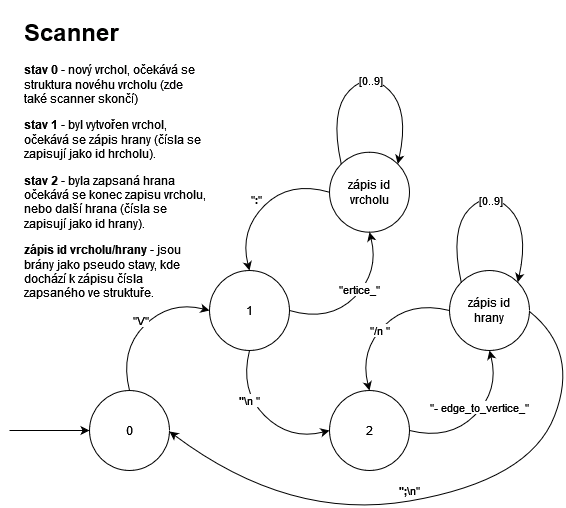
\includegraphics[width=0.9\textwidth]{doc/fig/Scanner_automat_Final.drawio.png}
    \caption{DKA}
    \label{fig:DKA}
\end{figure}


\newpage
